\begin{frame}{Learning to Intervene}
\begin{itemize}
\item Two feature sets:
\begin{itemize}
\item Metrics from \textbf{The Intervention Graph}
\item Plan distance measures from the sampled plans
\end{itemize}
\item Use the feature sets to train classifiers to recognize actions that should be flagged for intervention
\begin{itemize}
\item Naive Bayes, K-nearest neighbor, Decision tree, Logistic regression
\end{itemize}
\end{itemize}

\end{frame}


\begin{frame}{The Intervention Graph}
\begin{itemize}
\item Produce the intervention graph from current state (root) to $G_1$ (BAD) and $G_0$ (TAD) (leaves)
\end{itemize}

\begin{figure}[tb]
        \centering{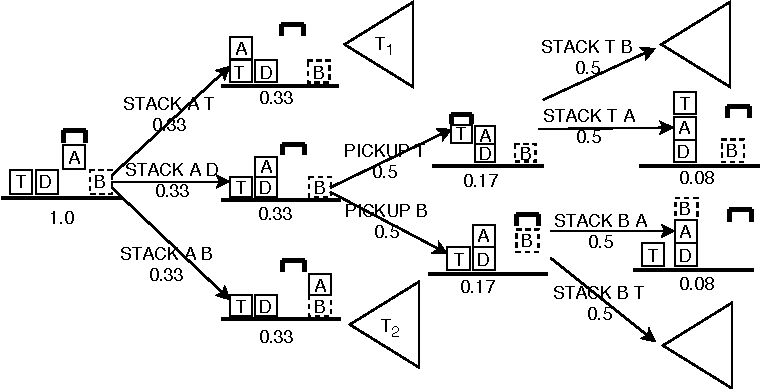
\includegraphics[width=\columnwidth]{img/featuresbw.pdf}}
\end{figure} 

\end{frame}


\begin{frame} {Intervention Graph Features}
\begin{itemize}
\item \textbf{Risk} - Posterior probability of reaching $G_1$, when the user is trying to reach $G_0$
\item \textbf{Desirability} - Posterior probability of reaching $G_0$, without passing $G_1$
\item \textbf{Distance to} $G_0$ - Mean number of edges between the root of the tree and $G_0$, which doesn't pass through $G_1$
\item \textbf{Distance to} $G_1$ - Mean number of edges between the root of the tree and $G_1$
\item \textbf{Active attack landmarks\%} - From the total number of predicates that must be true in any valid solution to the planning problem $\langle M,G_1\rangle$, how many are true in the current state?
\end{itemize}

\end{frame}

\begin{frame} {Plan Distance Measures From Sampled Plans}
\begin{itemize}
\item Instead of computing exact distances and probabilities \textbf{compute an estimated proximity} to $G_0$ and $G_1$
\item Use an automated planner to find two sets of solutions for $\langle M, G_0\rangle$ and $\langle M, G_1 \rangle$
\item Compute a \textbf{reference plan} $ = \lbrace observations + \pi_* \rbrace$
\item Compute the plan distances between the  \textbf{reference plan} and the plans in $\langle M, G_0\rangle$ and $\langle M, G_1 \rangle$
\end{itemize}

\end{frame}